\chapter{Gestión de cambios}

\section{Diagrama}
El equipo de desarrollo respeta el el flujo de trabajo representado en la figura \ref{fig:gdcambios}, para lograr el correcto seguimiento de una solicitud, añadiendo trazabilidad y credibilidad al proceso.
El proceso inicia con un documento estandarizado que detallamos en la ultima sección de este capitulo.

\begin{figure}[H]
    \centering
    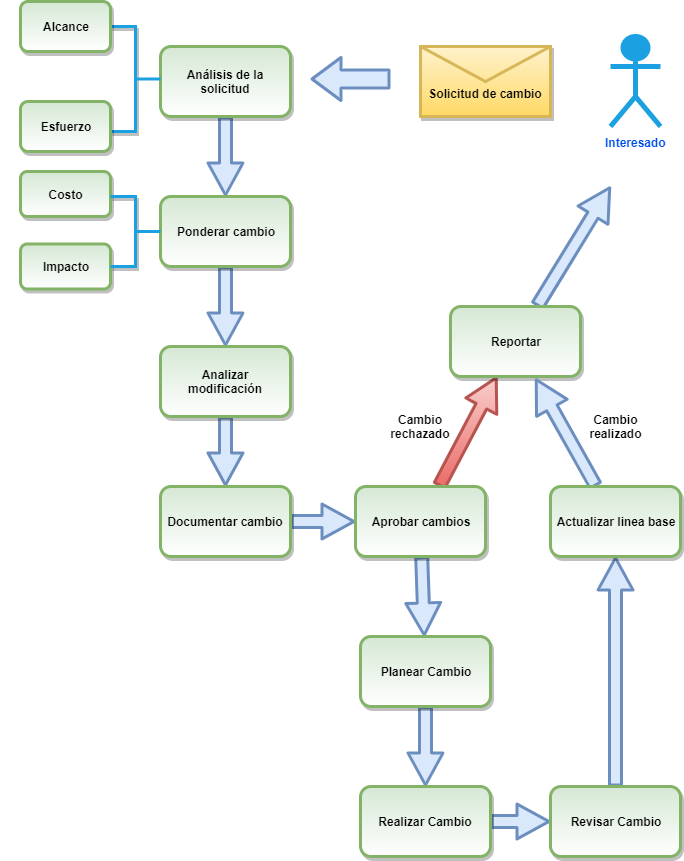
\includegraphics[scale=0.4]{Files/gestCambiosv2.png}
    \caption{Flujo de aceptación de cambio}
    \label{fig:gdcambios}
\end{figure}



\newpage
\section{Descripción}

\subsubsection{Se describe cada una de las tareas del proceso:}

\begin{itemize}
    \item Análisis de la solicitud
    \begin{itemize}
        \item La solicitud luego de ser recibida comienza a ser analizada en este punto, en esta etapa, los ítem más importantes a ser revisados son el alcance y el tiempo.
    \end{itemize}
    \item Valoración del cambio
    \begin{itemize}
        \item En este momento se analiza la trazabilidad del requisito, esto es, ver como le afecta el cambio de requisito a otros que estén relacionados, evaluando los costos que genera y el impacto que tiene en el software.
    \end{itemize}
    \item Análisis de la modificación
    \begin{itemize}
        \item En este punto se realiza un análisis más específico de el cambio, el encargado de realizar la implementación, o del equipo que realizará la implementación analiza técnicamente que otros cambios se deben realizar para cumplir con el requisito.
    \end{itemize}
    \item Documentación de la modificación
    \begin{itemize}
        \item En este momento se realiza la documentación de la solicitud del cambio, esta debe ser clara y no tener ambigüedades, debe contener además de la especificación, cual es el motivo del cambio y quien lo aprobó
    \end{itemize}
    \item Aprobación del cambio
    \begin{itemize}
        \item A partir de este momento se comienza a negociar con el cliente, si se continúa con la actividad de realizar el cambio o se vuelve a definir el cambio
    \end{itemize}
    \item Planear cambio
    \begin{itemize}
        \item Luego de la aprobación formal del cambio se planea el tiempo necesario y los recursos a utilizar
    \end{itemize}
    \item Realizar cambio
    \begin{itemize}
        \item En este punto se toman los recursos que se asignaron y se dispone a ejecutar la modificación
    \end{itemize}
    \item Revisar cambio
    \begin{itemize}
        \item Luego de que el cambio sea realizado se revisa si el trabajo hecho corresponde con los requisitos solicitados y aprobados previamente
    \end{itemize}
    \item Actualizar la linea base
    \begin{itemize}
        \item Se actualiza la línea base para que se continúe trabajando en el siguiente requisito
    \end{itemize}
    \item Informar
    \begin{itemize}
        \item Una vez que se realiza la modificación, se le debe comunicar al cliente que el cambio ha sido realizado, para que este lo verifique
    \end{itemize}
\end{itemize}

\section{Formulario de solicitud}

\subsubsection{Estándar de documento para solicitud de cambio:}

\prettyTable{|p{3cm}|p{4cm}|p{3cm}|p{4cm}|}{
    \textbf{Nro. Solicitud} &  & \textbf{Fecha} &   \\ \hline
    \textbf{Objetivo} &  & \textbf{Aplicación} &  \\ \hline
    \textbf{Interesado} & \multicolumn{3}{l|}{} \\ \hline
    \multicolumn{4}{|l|}{\mlcell{\textbf{Descripción de la modificación deseada:}\\ \\ 
                                                                                    \\
                                                                                    \\
                                                                                    \\
                                                                                    }} \\ \hline
    \multicolumn{4}{|l|}{\mlcell{\textbf{Motivo de la modificación:}\\ \\ 
                                                                                    \\
                                                                                    \\
                                                                                    \\
                                                                                    }} \\ \hline
}

\subsubsection{Detalle:}

\begin{itemize}
    \item Nro. de solicitud
    \begin{itemize}
        \item Indica el número correlativo de solicitud para poder identificado fácilmente
    \end{itemize}
    \item Fecha
    \begin{itemize}
        \item Indica la fecha en que fue solicitado el cambio
    \end{itemize}
    \item Objetivo
    \begin{itemize}
        \item Indica el objetivo principal por el cual es solicitado el cambio, ejemplo: regulación, optimización, etc.
    \end{itemize}
    \item Aplicación
    \begin{itemize}
        \item Indica a que aplicación de software es solicitado el cambio
    \end{itemize}
    \item Interesado
    \begin{itemize}
        \item Nombre o cargo de la persona que solicita el cambio
    \end{itemize}
    \item Descripción de la modificación deseada
    \begin{itemize}
        \item En esta campo se debe especificar con el mayor detalle posible, la modificación que se esta solicitando
    \end{itemize}
    \item Motivo de la modificación:
    \begin{itemize}
        \item Campo en el cual se debe indicar el motivo final del cambio, vital para la ponderación.
    \end{itemize}
\end{itemize}

\begin{comment}
     Identificación Control de cambios

Para una correcta identificación de lo controles de cambios de los requerimientos de las organizaciones de desarrollo de software, se identifican las siguientes actividades: 


·         Análisis de la Solicitud:

La solicitud es recibida por parte del cliente interno o externo, esta debe ser recibida por parte del líder de implementación para ser analizada. Uno de los puntos importantes para analizar son el Alcance y el Tiempo, esto con el fin de identificar si la solicitud es viable realizarla sobre el mismo requerimiento o si por el contrario es mejor manejarla como un requerimiento nuevo.

 Con respecto al análisis con relación al alcance es recomendable buscar colaboración con las áreas involucradas en la solicitud, para identificar de mejor manera el impacto y los elementos que se ven afectados con la solicitud.
 
 
 ·         Valorar el cambio

 Otro punto importante es valorar la factibilidad de la solicitud realizada ya sea por un cliente interno o uno externo. Para ello se deberá ir recorriendo todo el árbol de requisitos viendo como les afecta el cambio, y aquí es donde entra la trazabilidad de los requisitos.
 
 
 ·         Analizar Modificación

El líder de implementación debe realizar el análisis de la solicitud para saber que tanto impacta la modificación e identificar puntualmente las modificaciones solicitadas que afectan el requerimiento completo y así identificar si el cambio afecta mas de un requerimiento.
 
 
 ·         Documentar Cambio

Para tener un mejor control sobre los cambios solicitados es recomendable realizar una documentación clara para evitar ambigüedades en las modificaciones que se van a realizar a los requerimientos. Este punto apoya también a tener un control de las modificaciones que se realizan sobre un documento de requerimiento esto con el fin de mantener informado al grupo de trabajo y al cliente que actualizaciones se han realizado sobre los documentos, cual es la razón del cambio y quien lo aprobó. 
Aprobación Control de Cambios


·Aprobar Cambios

 Una vez se ha analizado el impacto del cambio, se debe tomar una decisión. Si se acepta el cambio, tras negociarlo con el cliente, se continuará con la actividad de implementar el cambio. En caso contrario, se deberá negociar con el cliente el siguiente paso a realizar.
 
 
 ·         Planear Cambio

 Después de tener una aprobación formal del cambio aceptado se planea el tiempo necesario y los recursos necesarios para llevar a cabo el cambio aprobado.
 
 
 ·         Realizar Cambio

 Una vez se planea el cambio aprobado se debe realizar las modificaciones necesarias a todos los productos que resulten afectados por dicho cambio.
 
 
 ·         Revisar Cambio

 Una vez se realice el cambio es recomendable hacer una verificación por parte del líder para identificar que el requerimiento incluye todos los cambios solicitados y que fueron aprobados.
 
 
 ·         Actualizar Línea Base

 Es recomendable utilizar el nuevo requerimiento como línea base, esto con el fin de trabajar siempre sobre la ultima versión del requerimiento.
 
 
 ·         Informar

 Una vez se realice la modificación de la solicitud se debe informar a los interesados que el cambio ya esta realizado para que sea verificado por el cliente.
\end{comment}